\section{\Sys Design}
\label{sec:methodology}

% \begin{algorithm}[h]
%   \scriptsize
%   \DontPrintSemicolon
%   \SetKwInOut{Input}{Inputs}
%   \SetKwInOut{Output}{Output}
%   \Input{Set of client models $\{M_1, M_2, \ldots, M_N\}$;\\}
%   \Output{Global GNN model $G$.}
%   \BlankLine
%   \tcc{Initialize global GNN model with random weights.}
%   $G \leftarrow \text{InitializeRandomWeights}()$\\
%   \tcc{Distribute $G$ to all clients.}
%   \ForEach{client model $M_i$}{
%     Send $G$ to $M_i$\\
%     $G_i \leftarrow \text{TrainOnLocalData}(M_i)$
%   }
%   \BlankLine
%   \tcc{Aggregate trained models from clients.}
%   $AggregatedWeights \leftarrow list([])$\\
%   \ForEach{client model $G_i$}{
%     $AggregatedWeights.append(\text{ExtractWeights}(G_i))$\\
%   }
%   \tcc{Apply federated averaging.}
%   $G \leftarrow \text{FederatedAveraging}(AggregatedWeights)$\\
%   \BlankLine
%   \Return $G$\\
%   \BlankLine
%   \caption{Federated Graph Representation Learning}
%   \label{alg:federated_learning}
% \end{algorithm}

\begin{algorithm}[!t]
  \scriptsize
  \DontPrintSemicolon
  \SetKwInOut{Input}{Inputs}
  \SetKwInOut{Output}{Output}
  \Input{Set of client models $\{M_1, M_2, \ldots, M_N\}$; Privacy parameter $\epsilon$.}
  \Output{Global GNN model $G$.}
  \BlankLine
  \tcc{Initialize global GNN model with random weights.}
  $G \leftarrow \text{InitializeRandomWeights}()$\\
  \tcc{Distribute $G$ to all clients.}
  \ForEach{client model $M_i$}{
    Send $G$ to $M_i$\\
    $G_i \leftarrow \text{TrainOnLocalData}(M_i)$\\
    $G_i \leftarrow \text{AddGaussianNoise}(\epsilon)$
  }
  \BlankLine
  \tcc{Aggregate privacy-preserving trained models from clients.}
  $AggregatedWeights \leftarrow list([])$\\
  \ForEach{client model $G_i$}{
    $AggregatedWeights.append(\text{ExtractWeights}(G_i))$\\
  }
  $G \leftarrow \text{FederatedAveraging}(AggregatedWeights)$\\
  \BlankLine
  \Return $G$\\
  \BlankLine
  \caption{Federated Graph Representation Learning.}
  \label{alg:federated_learning}
\end{algorithm}

In this section, we detail the architecture of \Sys, which is composed of six key modules. The architecture begins with the \textit{Provenance Graph Constructor} module on each client machine, transforming audit logs into a provenance graph. Following this, the \textit{Semantic Featurization} module encodes semantic attributes from the audit logs into feature vectors, facilitating the training of client-specific \gnnshort models.

The \textit{Semantic Vectors Harmonization} module aims to privately consolidate individual client word2vec models into a cohesive global model, employing a trusted utility server and encryption techniques to ensure the privacy of model data.

Next, the \textit{System Entity Categorization} module categorizes all system entities across clients into standardized categories, promoting uniformity in the training of \gnnshort models.

The \textit{Federated Graph Learning Module} proceeds to train \gnnshort models by these categories on each client machine, using the harmonized semantic features. After training, the models are sent to a central server for federated learning, where the federated averaging algorithm integrates the models based on the system entity categories they were trained on.

Lastly, the \textit{Anomaly Detection Module} employs the unified global models for anomaly detection on each client machine. Figure \ref{fig:arch} presents the comprehensive architecture of \Sys, with further details in the subsequent subsections:

\begin{figure*}[t!]
  \centering
  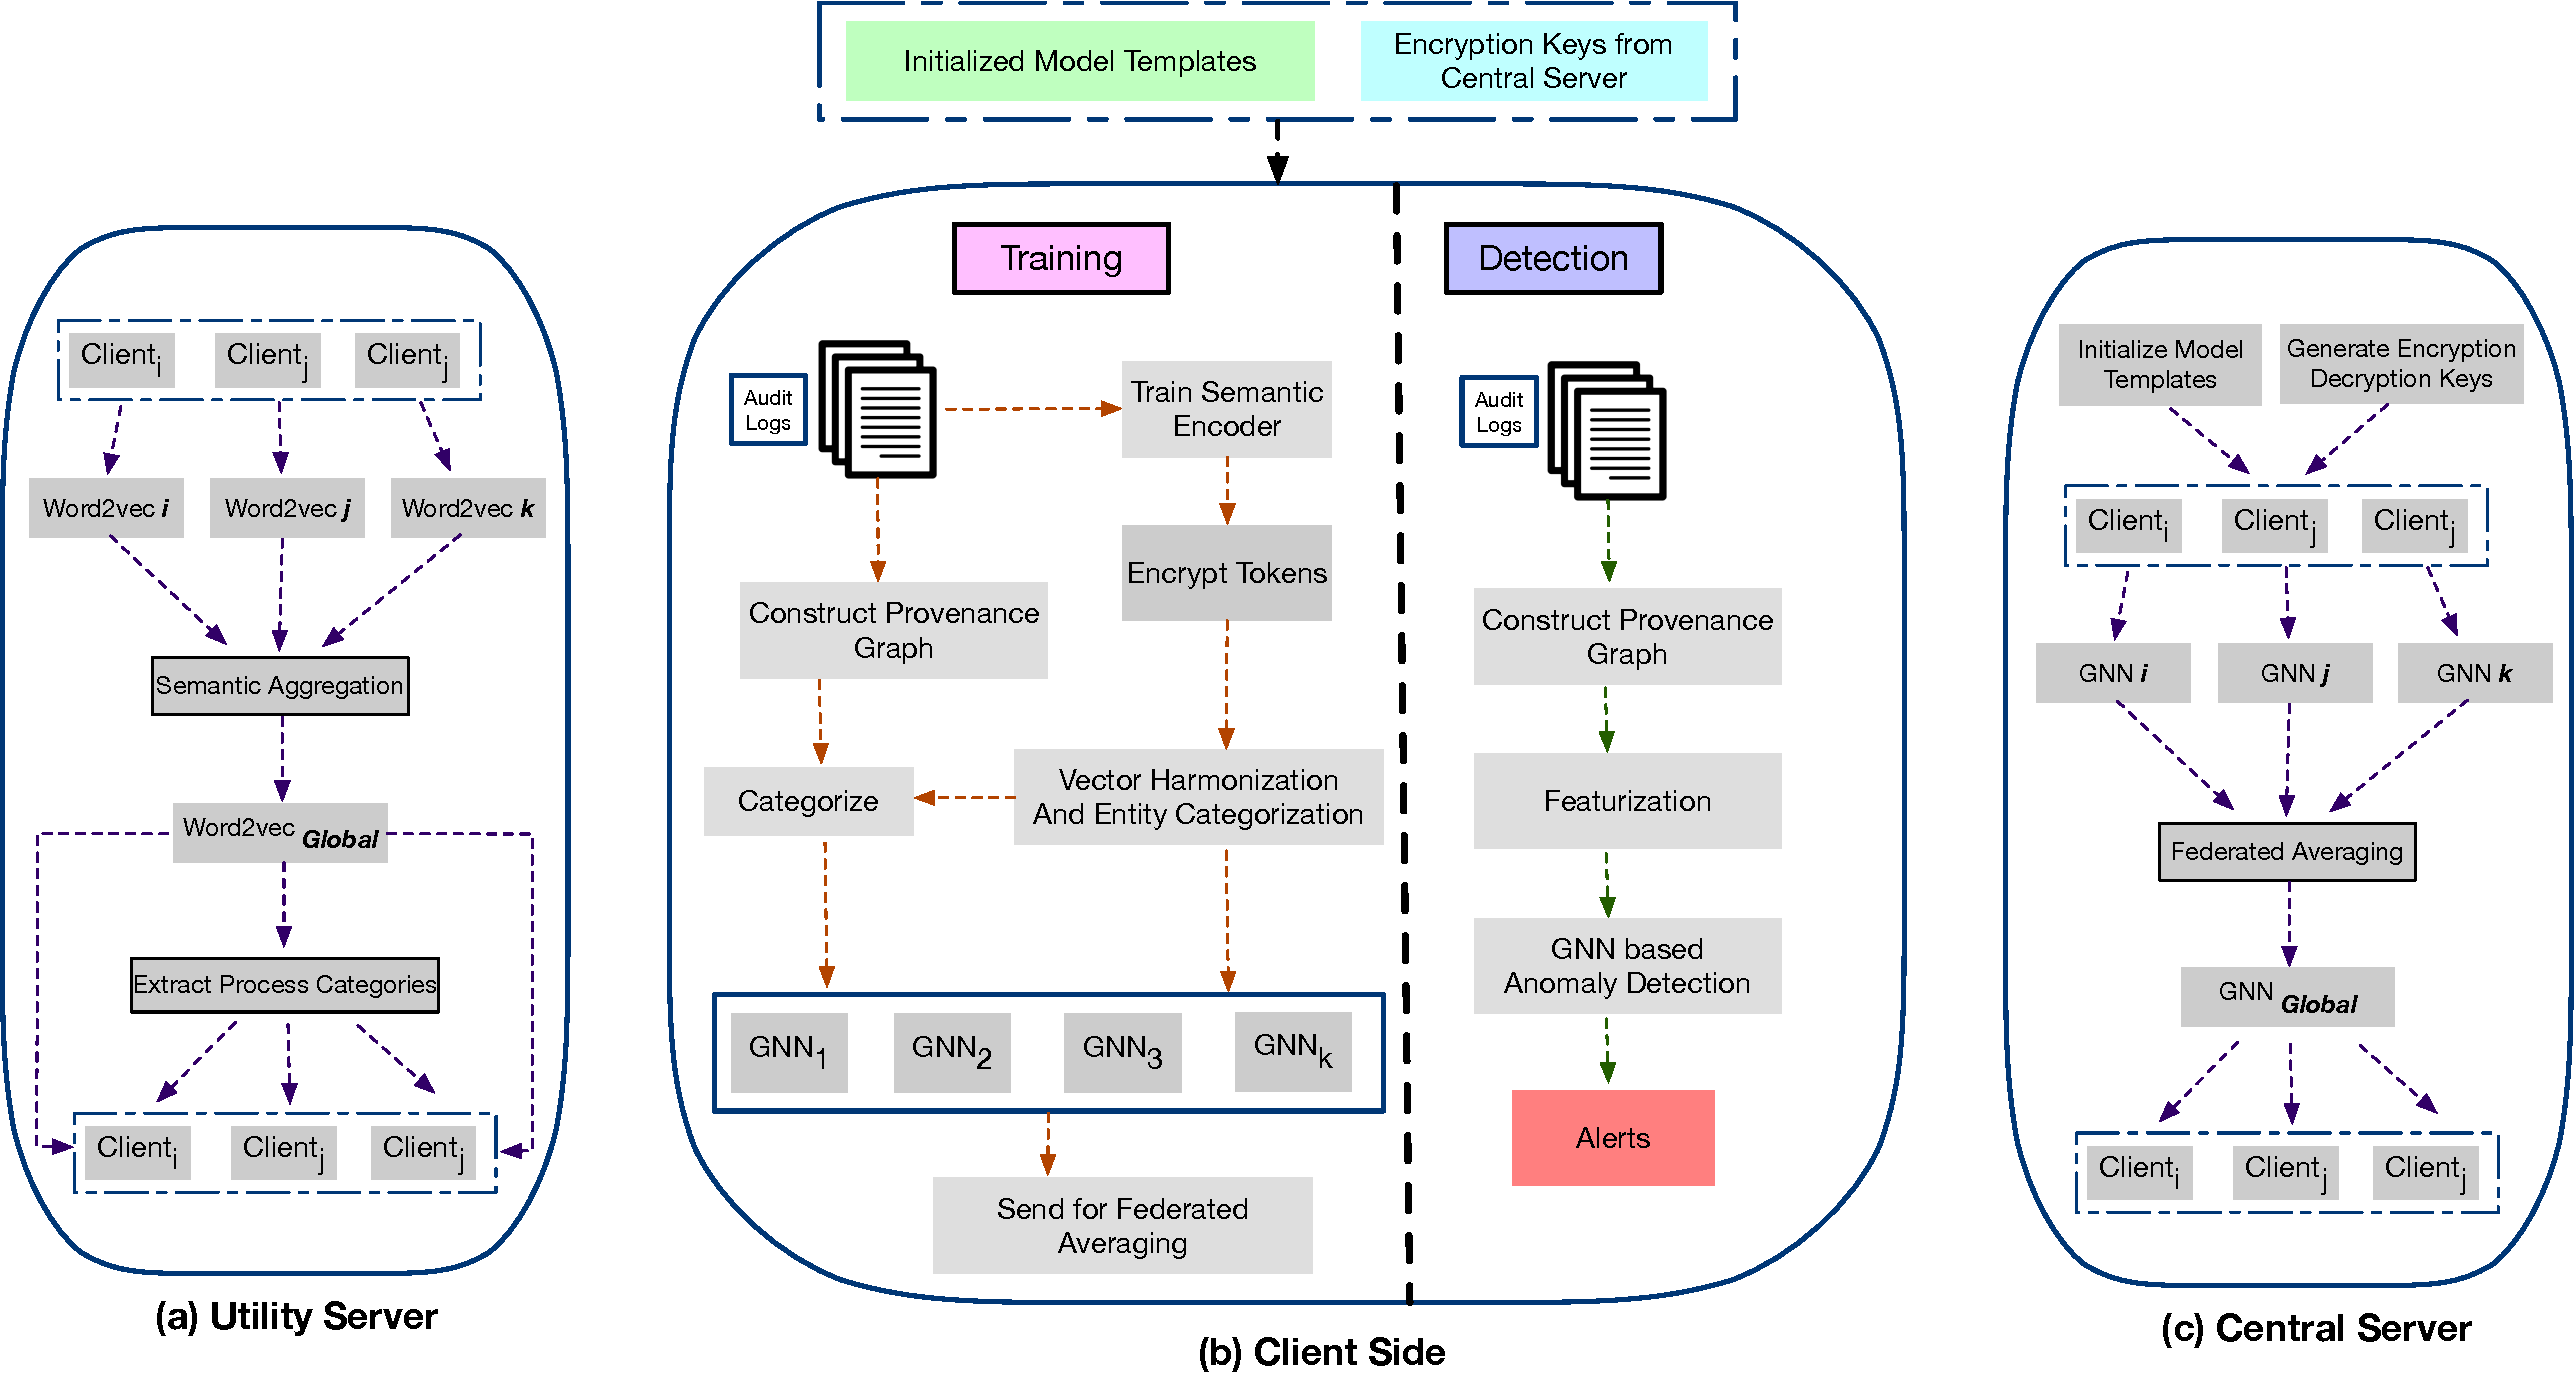
\includegraphics[width=\textwidth]{fig/archv2.pdf}
  \caption{High Level Architecture of \Sys.}
  \vspace{-3ex}
  \label{fig:arch}
\end{figure*}


\subsection{Provenance Graph Constructor} 
Sys utilizes audit logs to construct a system provenance graph. It operates on each client machine, using their local system logs to build the graph. Major operating systems, including Linux and Windows, come equipped with built-in mechanisms for log collection—specifically, the Linux Audit system and Windows Event Tracing. These logs provide detailed insights into the interactions among various system entities, capturing activities such as process executions, file operations, and network connections. Using this data, Sys forms a graph where nodes represent system entities including processes, files, and sockets. The edges of this graph denote events, identified by syscalls, that occur between these entities. Moreover, Sys enhances each node with comprehensive attributes, including process names, command lines, file names, and network IP addresses. As demonstrated by prior works~\cite{flash2024,cheng2023kairos}, these contextual attributes enable the model to develop a robust understanding of system behavior.

\subsection{Semantic Featurization}

This module processes the provenance graph generated from audit logs by transforming node attributes into feature vectors for the graph learning phase. Systems like Flash have demonstrated the effectiveness of using semantic node attributes to enhance detection performance. Building on this approach, we employ a word2vec language model to encode these attributes into vector format, \(\mathbf{v}\), where each attribute \(a\) is transformed into a vector \(v_a\). Each client independently trains a word2vec model using their local system logs. The transformation of an attribute \(a\) into a vector by the word2vec model can be represented as:

\[
v_a = \text{Word2Vec}(a)
\]

However, before these models can be utilized to encode text attributes, they must be merged across client machines to form a unified model. This unification is crucial; without it, each client would produce differing feature vectors, \(v_a^i\), for identical inputs, where \(i\) indicates the client. The variability in feature vectors, \(\{v_a^1, v_a^2, \ldots, v_a^N\}\), for the same attribute \(a\) across \(N\) clients, would undermine the consistency of client-based GNN models. To ensure uniformity, the feature vectors for overlapping attributes must be averaged across clients, forming a single unified vector for each attribute:

\[
\bar{v}_a = \frac{1}{N} \sum_{i=1}^{N} v_a^i
\]

Such averaging ensures consistency in the feature representation, enhancing the effectiveness of the federated averaging technique by maintaining uniformity in the input space for the GNN models across all clients.


\subsection{Semantic Vectors Harmonization}
This module integrates individual client word2vec models into a unified model for use across all clients. The word2vec model functions as a key-value store, with vocabulary tokens as keys, \(k\), and their corresponding vector representations as values, \(v_k\). To combine these models, we calculate the average vector of overlapping tokens from all client machines, creating a central model. The mathematical representation for averaging vectors of a token \(k\) across \(N\) clients is given by:

\[
\bar{v}_k = \frac{1}{N} \sum_{i=1}^{N} v_{k,i}
\]

where \(\bar{v}_k\) is the averaged vector for token \(k\), and \(v_{k,i}\) is the vector representation of token \(k\) from the \(i\)-th client model.

However, transferring tokens—containing sensitive data like process names, file names, and IP addresses—to a central server could breach user privacy. To mitigate this, we employ a trusted utility server. Initially, the central server distributes an encryption key, \(E\), and a decryption key, \(D\), pair to each client. Clients then encrypt their word2vec model tokens using the encryption key:

\[
E(v_{k}) = v_{k}^{'}
\]

and send them to the utility server. This server merges the encrypted models and dispatches the unified model back to the clients, who decrypt it using the decryption key:

\[
D(v_{k}^{'}) = v_{k}
\]

This procedure ensures that neither the central server nor the utility server can access the actual token information, assuming no collusion between the two servers. The process is explained in detailed in algorithm~\ref{alg:secure_integration_averaging_word2vec}

\begin{algorithm}[!t]
  \scriptsize
  \DontPrintSemicolon
  \SetKwInOut{Input}{Inputs}
  \SetKwInOut{Output}{Output}
  \Input{Client Word2Vec models $\{M_1, M_2, \ldots, M_N\}$ encrypted with key $E$; Encryption key $E$; Decryption key $D$.}
  \Output{Encrypted unified Word2Vec model $U'$ sent to clients.}
  \BlankLine
  \tcc{Distribute encryption and decryption keys to each client.}
  \ForEach{client $C_i$}{
    Send $E$ and $D$ to $C_i$\\
  }
  \tcc{Clients encrypt their model tokens.}
  \ForEach{client model $M_i$}{
    $M_i' \leftarrow$ EncryptModelTokens($M_i$, $E$) \tcc*{Encrypt tokens using $E$.}
    Send $M_i'$ to Utility Server\\
  }
  \tcc{Utility server merges encrypted models.}
  $TokenVectors \leftarrow$ InitializeEmptyDictionary()\\
  $TokenCounts \leftarrow$ InitializeEmptyDictionary()\\
  \ForEach{encrypted model $M_i'$}{
    \ForEach{token $t$ in $M_i'$}{
      $Vector \leftarrow M_i'[t]$\\
      \eIf{$TokenVectors$.HasKey($t$)}{
        $TokenVectors[t] \leftarrow TokenVectors[t] + Vector$\\
        $TokenCounts[t] \leftarrow TokenCounts[t] + 1$\\
      }{
        $TokenVectors[t] \leftarrow Vector$\\
        $TokenCounts[t] \leftarrow 1$\\
      }
    }
  }
  \tcc{Average the vectors for overlapping tokens.}
  \ForEach{token $t$ in $TokenVectors$.Keys()}{
    $TokenVectors[t] \leftarrow TokenVectors[t] / TokenCounts[t]$\\
  }
  $U' \leftarrow$ NewModel($TokenVectors$, $EncryptedTokens$) \tcc*{Constructing a new unified model.}
  \ForEach{client $C_i$}{
    Send $U'$ to $C_i$\\
  }
  \BlankLine
  \Return{Harmonized model $U'$ has been dispatched to all clients.}\\
  \BlankLine
  \caption{Secure Integration and Averaging of Word2Vec Models}
  \label{alg:secure_integration_averaging_word2vec}
\end{algorithm}

\subsection{Federated Graph Learning}
% The module performs graph representation learning in a federated manner. It includes a central server responsible for initializing a global \gnnshort model with random weights, which is then sent to all clients. These clients use their local provenance graphs and semantic feature vectors to train the \gnnshort model in an unsupervised way, following a training method similar to Flash. The \gnnshort model's objective is to classify each node entity into its corresponding type. After training their models, the clients send them back to the central server. The server applies the federated averaging algorithm to merge these models into a single global model. The server aggregates parameters from $N$ client models to update the global model as follows:
% \[
% \bar{w} = \frac{1}{N} \sum_{k=1}^{N} w_k
% \]

% where:
% \begin{itemize}
%     \item $\bar{w}$ is the aggregated global model parameter.
%     \item $N$ is the number of client models.
%     \item $w_k$ is the parameter from the $k$-th client model.
% \end{itemize}

% This formula averages the parameters of all client models, forming the global model update. The process is repeated for a set number of rounds, determined by a hyperparameter, and concludes when there is no further reduction in training loss. Algorithm~\ref{alg:federated_learning} explains this process in detail.

The module performs graph representation learning in a federated manner. It includes a central server responsible for initializing a global \texttt{GNN} model with random weights, which is then sent to all clients. These clients use their local provenance graphs and semantic feature vectors to train the \texttt{GNN} model in an unsupervised way, following a training method similar to Flash. The \texttt{GNN} model's objective is to classify each node entity into its corresponding type. After training their models, the clients apply local differential privacy (LDP) to their model updates by adding a placeholder for Gaussian noise parameterized by \(\epsilon\). This ensures the privacy of their updates before sending them back to the central server. The server then applies the federated averaging algorithm to merge these privacy-preserving models into a single global model. Specifically, the server aggregates parameters from \(N\) client models, incorporating the Gaussian noise, to update the global model as follows:

\begin{equation}
\bar{w} = \frac{1}{N} \sum_{k=1}^{N} \left(w_k + \text{G}(\epsilon)\right)
\end{equation}

where:
\begin{itemize}
    \item \(\bar{w}\) is the aggregated global model parameter.
    \item \(N\) is the number of client models.
    \item \(w_k\) is the parameter from the \(k\)-th client model.
    \item \(\text{G}(\epsilon)\) is the the Gaussian noise added to each client's model parameters, parameterized by \(\epsilon\).
\end{itemize}

This approach not only averages the parameters of all client models but also ensures the privacy of each client's data by perturbing the model updates with noise parameterized by \(\epsilon\). The process is repeated for a set number of rounds, determined by a hyperparameter, and concludes when there is no further reduction in training loss. Algorithm~\ref{alg:federated_learning} explains this process in detail, including the application of local differential privacy.

\subsection{Anomaly Detection}
\Sys employs an advanced methodology akin to systems like Flash and \threatrace, focusing on identifying irregular nodes through the comparison of their expected and observed types. This approach is grounded in a detailed analysis of both the surrounding structures and inherent properties of the nodes, with the aim to define normal pattern baselines for various node types. Typically, entities with malicious intentions display neighborhood configurations and characteristics deviating from these established norms. In operational phases, the detection of anomalies that diverge from the pre-established node distribution patterns often results in their misclassification. The emergence of nodes misclassified in the system's output is indicative of potential security issues. To regulate the frequency of alerts, we have implemented a threshold parameter, denoted as $T$. This parameter sets a limit on the likelihood of a classification being considered valid. A higher value of this parameter implies stronger confidence in the prediction, increasing the probability of identifying anomalies.

% \subsection{Provenance Graph Constructor}
% Our approach starts by converting system logs into provenance graphs through a three-step process. Initially, the system, \Sys, processes system logs like Windows Event Logs or Linux Audit Logs, which are composed of host event details including process activities, file interactions, and network engagements. \Sys works with batches of audit logs, utilizing a sliding window technique to create the provenance graph. This graph consists of two kinds of nodes: process nodes and object nodes. The object nodes represent various system entities such as files, network streams, modules, and other system components. The connections between these nodes are marked with labels indicating the event type, elucidating the cause-and-effect relationship among the connected nodes and the event's timestamp. Additionally, these nodes are equipped with attributes like process identifiers, command lines, file paths, IP addresses, port details, and module paths, offering additional insights and specifics.

% \subsection{Semantic Vectors Harmonization}
% \wajih{You need to add formalism in this subsection overall. If there is a Math related to Harmonization add that. Look into the Flash paper -- we gave so much internal details about the algorithms. }
% Our system employs the word2vec model to encode various semantic attributes into a vector space, which is pivotal in distinguishing normal system entities from anomalies. Traditional approaches utilize a centralized word2vec model for this encoding. However, in a federated learning context, complexities arise as each individual client must train its word2vec model for attribute encoding. Consequently, different clients might encode the same attributes into diverse vectors, leading to a non-Independent and Identically Distributed (Non-IID) problem. This variation hampers the convergence of the Graph Neural Network (GNN) model in federated learning scenarios. 

% To address this issue, we have developed a technique leveraging a utility server to synchronize disparate models across clients. This approach achieves uniformity in encoding the same attributes while preserving privacy, as clients are not required to share their attributes. The process initiates with the main server distributing an encryption and decryption key to each client. Clients then encrypt their word2vec model tokens, concealing their meanings. Subsequently, these encrypted models are sent to the utility server, which remains unaware of the encryption key used. The utility server then averages the vectors for the corresponding encrypted tokens, creating a unified and harmonized word2vec model. Finally, this model is returned to the clients, who utilize the decryption key to revert their encrypted tokens to their original attributes.

% \subsection{Federated Learning Module}
% \wajih{You need to add formalism in this subsection overall. If there is a Math related to FL add that. Look into the Flash paper -- we gave so much internal details about the algorithms. }
% Each client machine independently trains a \gnn model on a provenance graph built from its local log data, thereby preserving privacy. These individually trained models are then sent to the main server. Upon receiving them, the main server applies a federated averaging algorithm to integrate these models into a single, centralized model. This unified model is subsequently distributed back to each client. This cycle of training and unification is repeated over several rounds until the model reaches convergence. Finally, clients employ the fully trained model to perform anomaly detection.

% \subsection{Anomaly Detection}
% \wajih{Again missing scientific details about your approach.}
% \Sys utilizes an advanced approach similar to existing systems like Flash and \threatrace to pinpoint irregular nodes by assessing the disparity between their expected and observed types. This method is rooted in a thorough examination of the surrounding structures and intrinsic qualities of nodes, aiming to establish a baseline of normal patterns for various node classifications. It is observed that entities with malicious intent often manifest neighborhood configurations and characteristics that are inconsistent with these established norms. During operational phases, encountering such anomalies that stand apart from the pre-learned node distribution patterns leads to their erroneous classification. The presence of nodes incorrectly categorized in the output serves as an indicator of potential security concerns. We have introduced a regulatory mechanism in the form of a threshold parameter, $T$, to oversee the frequency of alerts. This parameter effectively caps the classification likelihood for a given prediction. A higher parameter value correlates with stronger conviction in the prediction, signaling a greater chance of uncovering anomalies.
